\chapter{Introduction}\label{C:intro}

Test suites are important part in every major project. They are created in an attempt to test a software program and show that it has some specified set of behaviours. This specified set of behaviours often examine a large number of code paths, so covering the majority can incur a large number of tests and in turn take several hours to run. Throughout the project test cases are constantly being added; when a piece of code is altered, new code is developed or a bug gets fixed \cite{issuetrack,whentotest}. A question arises, how can we ensure that the thousandth test case is not replicating the behaviour of the first? Even with careful planning, it is near impossible to have no redundant test cases. This is when a test is nearly or exactly a replication of another test. Therefore, examination of the information left behind during test execution should occur. 

During a test's execution, a paper trail is left behind. This trail contains information ranging from low level to high level run time data. The information that this research is interested in is the method execution details, referred to as the tests spectra. We can analyse this spectrum using different metrics to determine how related a test is to another and each test will be analysed with every other test. Using this analysed information, we can help identify potential redundant test cases. In Figure \ref{fig:spectra} we see a figurative spectra for three different tests where colours represent method executions. Intuitively, it is clear that Test 1 is different from Test 2 and 3. However, there appear to be similarities between Test 2 and 3 which may need further investigation.

\begin{figure}[h]
\centering
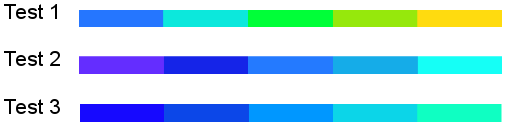
\includegraphics[width=6cm,height=3cm]{spectra.png}
\caption{A figurative spectra where each colour represents different method execution details. We see similarities between Test 2 and 3. In contrast, Test 1 is different from 2 and 3. }
\label{fig:spectra}
\end{figure}

It is important to understand the dangers of removing test cases. Unless two test cases are exactly the same, it is difficult to guarantee that they are redundant, even if one subsumes another. Therefore the aim of the project is to create a framework that gives developers different approaches in identifying redundant test cases. The framework should allow a developer to configure different analysis metrics and view the results on a graphical user interface (GUI). This means that the framework is useful for gaining an overview and understanding of the condition of the current test suite, allowing for manual inspection to determine if potentially redundant tests are redundant.

A potential use case of the framework is redistribute the test cases. This can be achieved through splitting of any closely redundant tests into separate test suites and running the suites at different times, ensuring that we are retaining the original bug finding ability. For example, one test suite can be run during continuous integration, and the other over night.

David Pearce is currently writing a language called Whiley, which contains an extended static checking framework in order to eliminate run time exceptions through formal verification techniques. In the compiler module alone, there are roughly 1500 tests. Relocating a number of these tests into another suite would result in allowing David Pearce to increase development speed due to a reduction in the time taken to run a large test suite. Running tests often allows for bugs to be traced back to code changes easier, using a smaller suite for every few changes means it will take less time to run. The bug finding ability is not affected due to being able to run the full suite when development is not being done. 